From HW~\ref{hw:mass}.\ref{chap:transfer_function_models}, the transfer function model is
\[
\tilde{Z}(s) = \frac{\frac{1}{m}}{s^2+\frac{b}{m}s+\frac{k}{m}}\tilde{F}(s) \defeq P(s)\tilde{F}(s).
\]
Figure~\ref{fig:hw_mass_compensator_design_1} shows the Bode plot for $P$ together with the design specification on tracking and attenuating the noise.  The requirement to reject constant input disturbances requires the inclusion of an integrator which is not shown in Figure~\ref{fig:hw_mass_compensator_design_1}.
%
\begin{figure}[H]
   \centering
   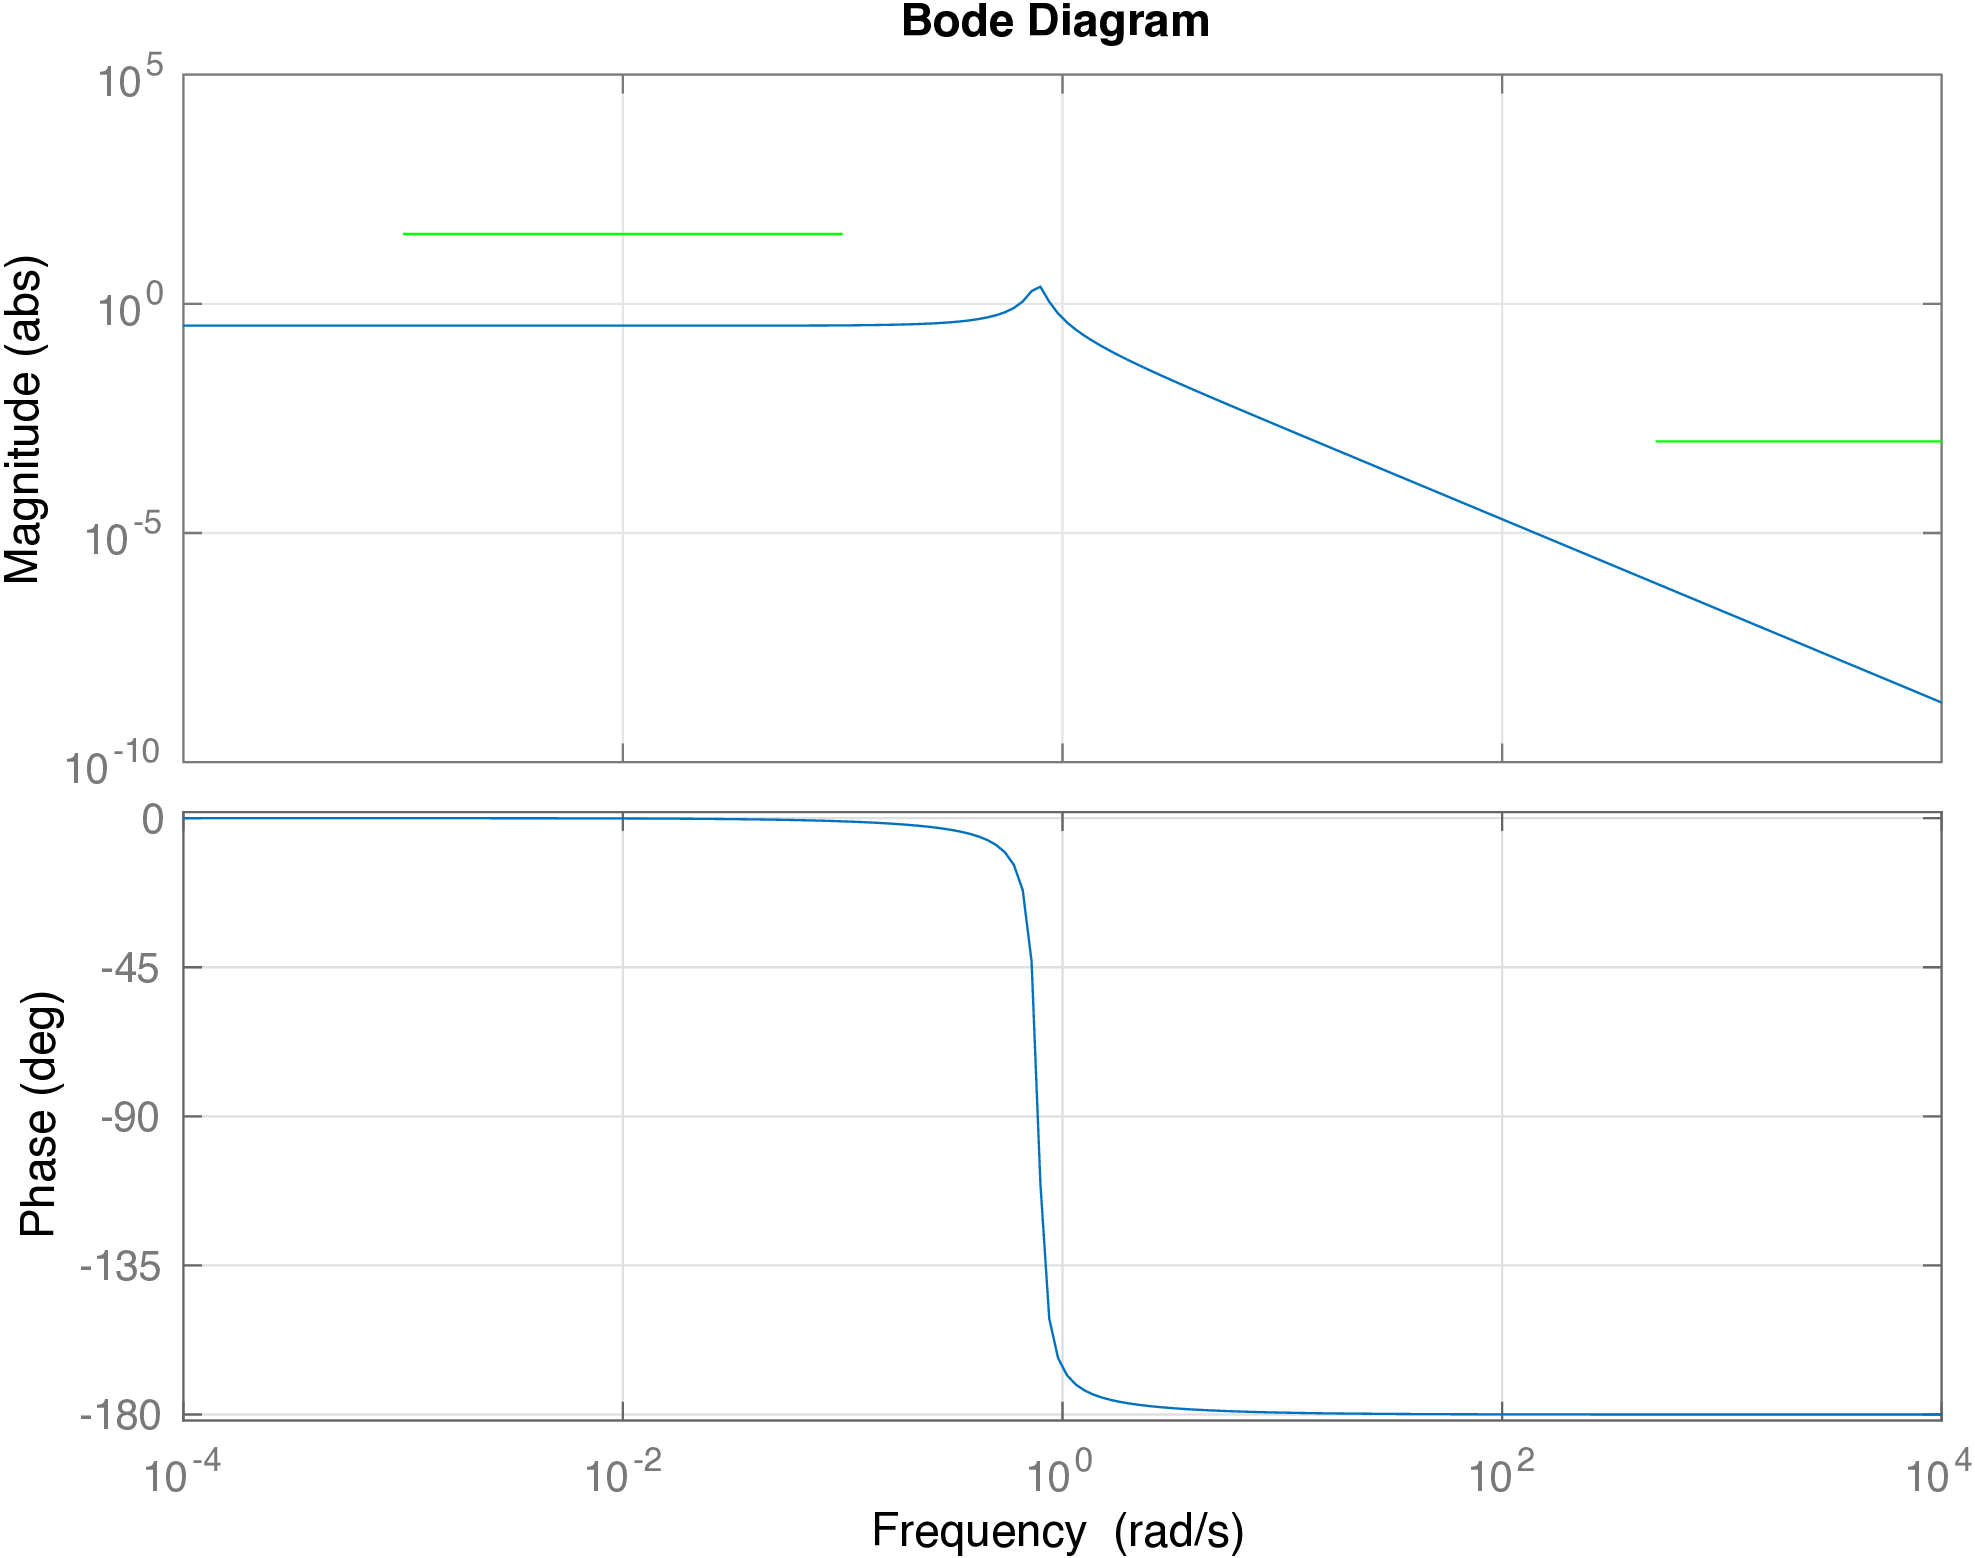
\includegraphics[width=0.95\textwidth]{6_design_studies/figures/hw_mass_compensator_design_1.pdf}
   \caption{The Bode plot for the plant in HW~\ref{hw:mass}.\ref{chap:loopshaping_design}, together with the design specifications.}
   \label{fig:hw_mass_compensator_design_1}
\end{figure}

The first step is to add PI compensation to meet the requirement on rejecting input disturbances.  Figure~\ref{fig:hw_mass_compensator_design_2} shows the loop gain after adding the PI control
\[
C_{int} = \frac{s+0.2}{s}.
\]
\begin{figure}[H]
   \centering
   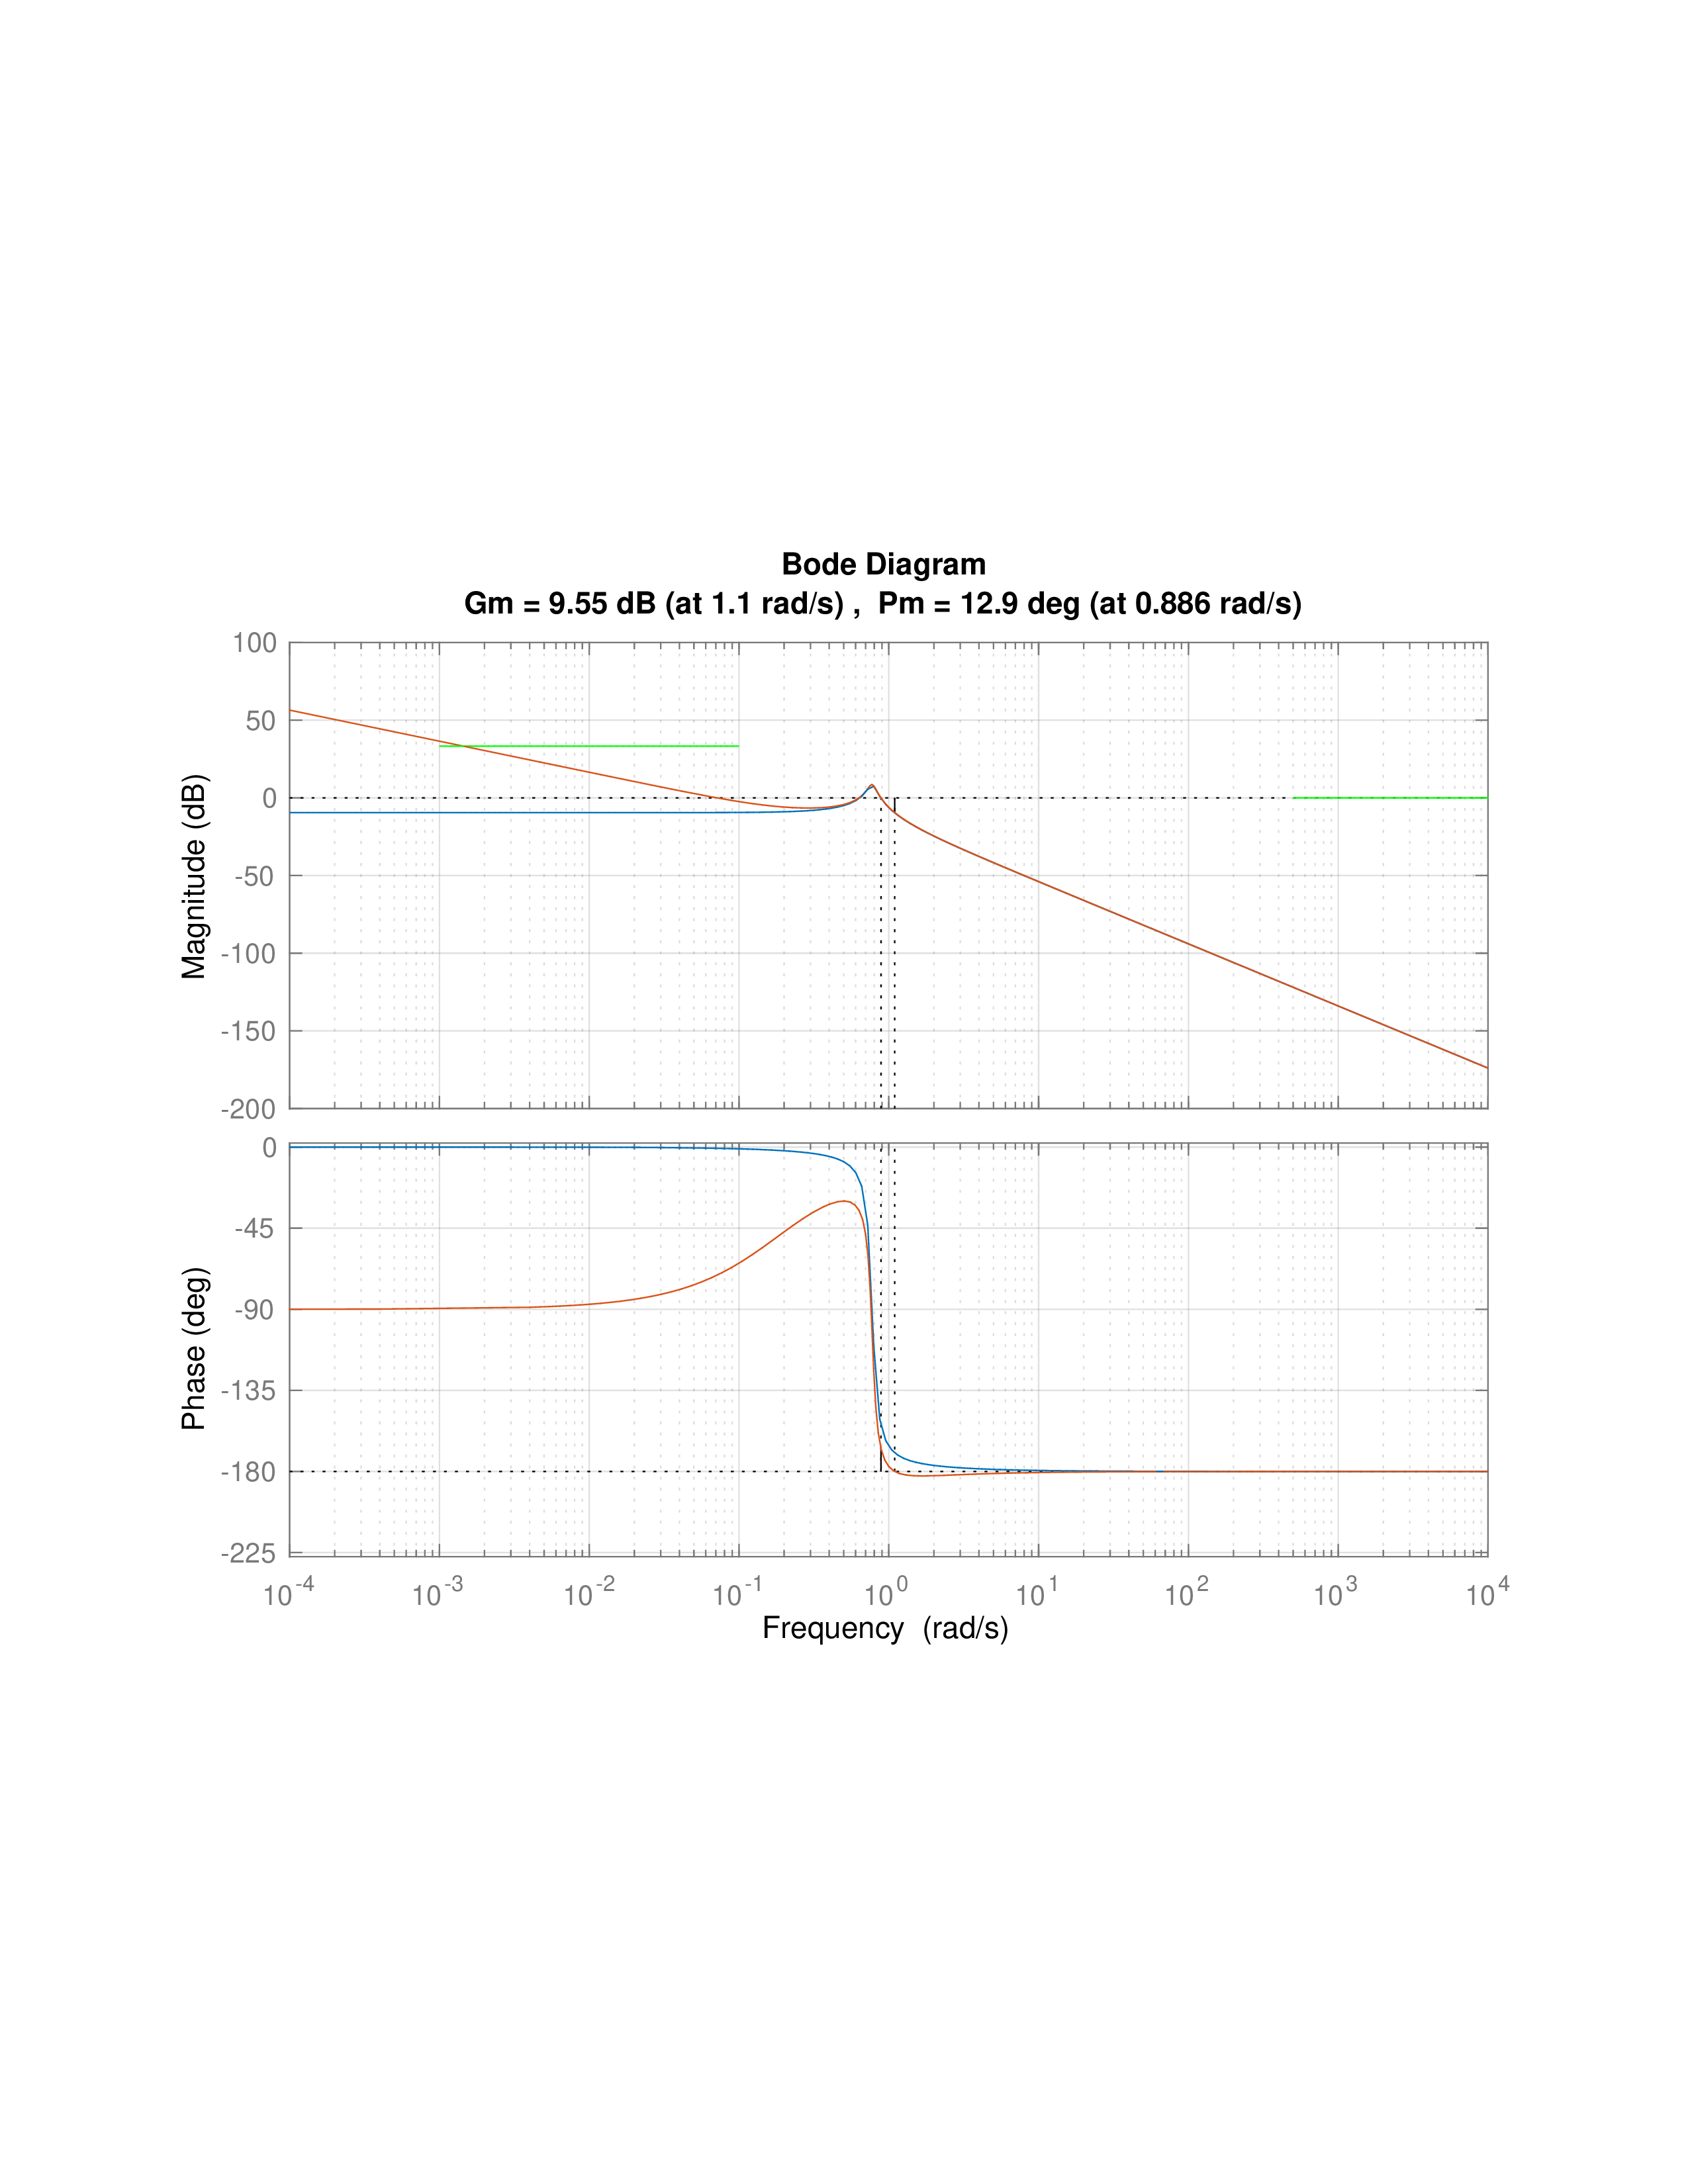
\includegraphics[width=0.95\textwidth]{6_design_studies/figures/hw_mass_compensator_design_2.pdf}
   \caption{The Bode plot for the outer loop system in HW~\ref{hw:mass}.\ref{chap:loopshaping_design}, with PI control.}
   \label{fig:hw_mass_compensator_design_2}
\end{figure}
Our goal is to cross over the system midway between the low and high frequency constraints. Let's choose $\omega_{co}$ = 7~rad/s. At this frequency, the PM is slightly negative. We will add 60~deg of PM to stabilize and add damping to the system. Figure~\ref{fig:hw_mass_compensator_design_3} shows the loopgain with the addition of the phase lead filter
\[
C_{lead} = \frac{s+1.88}{s+26.1},
\]
and the proportional gain $k_P=13.9$.
\begin{figure}[H]
   \centering
   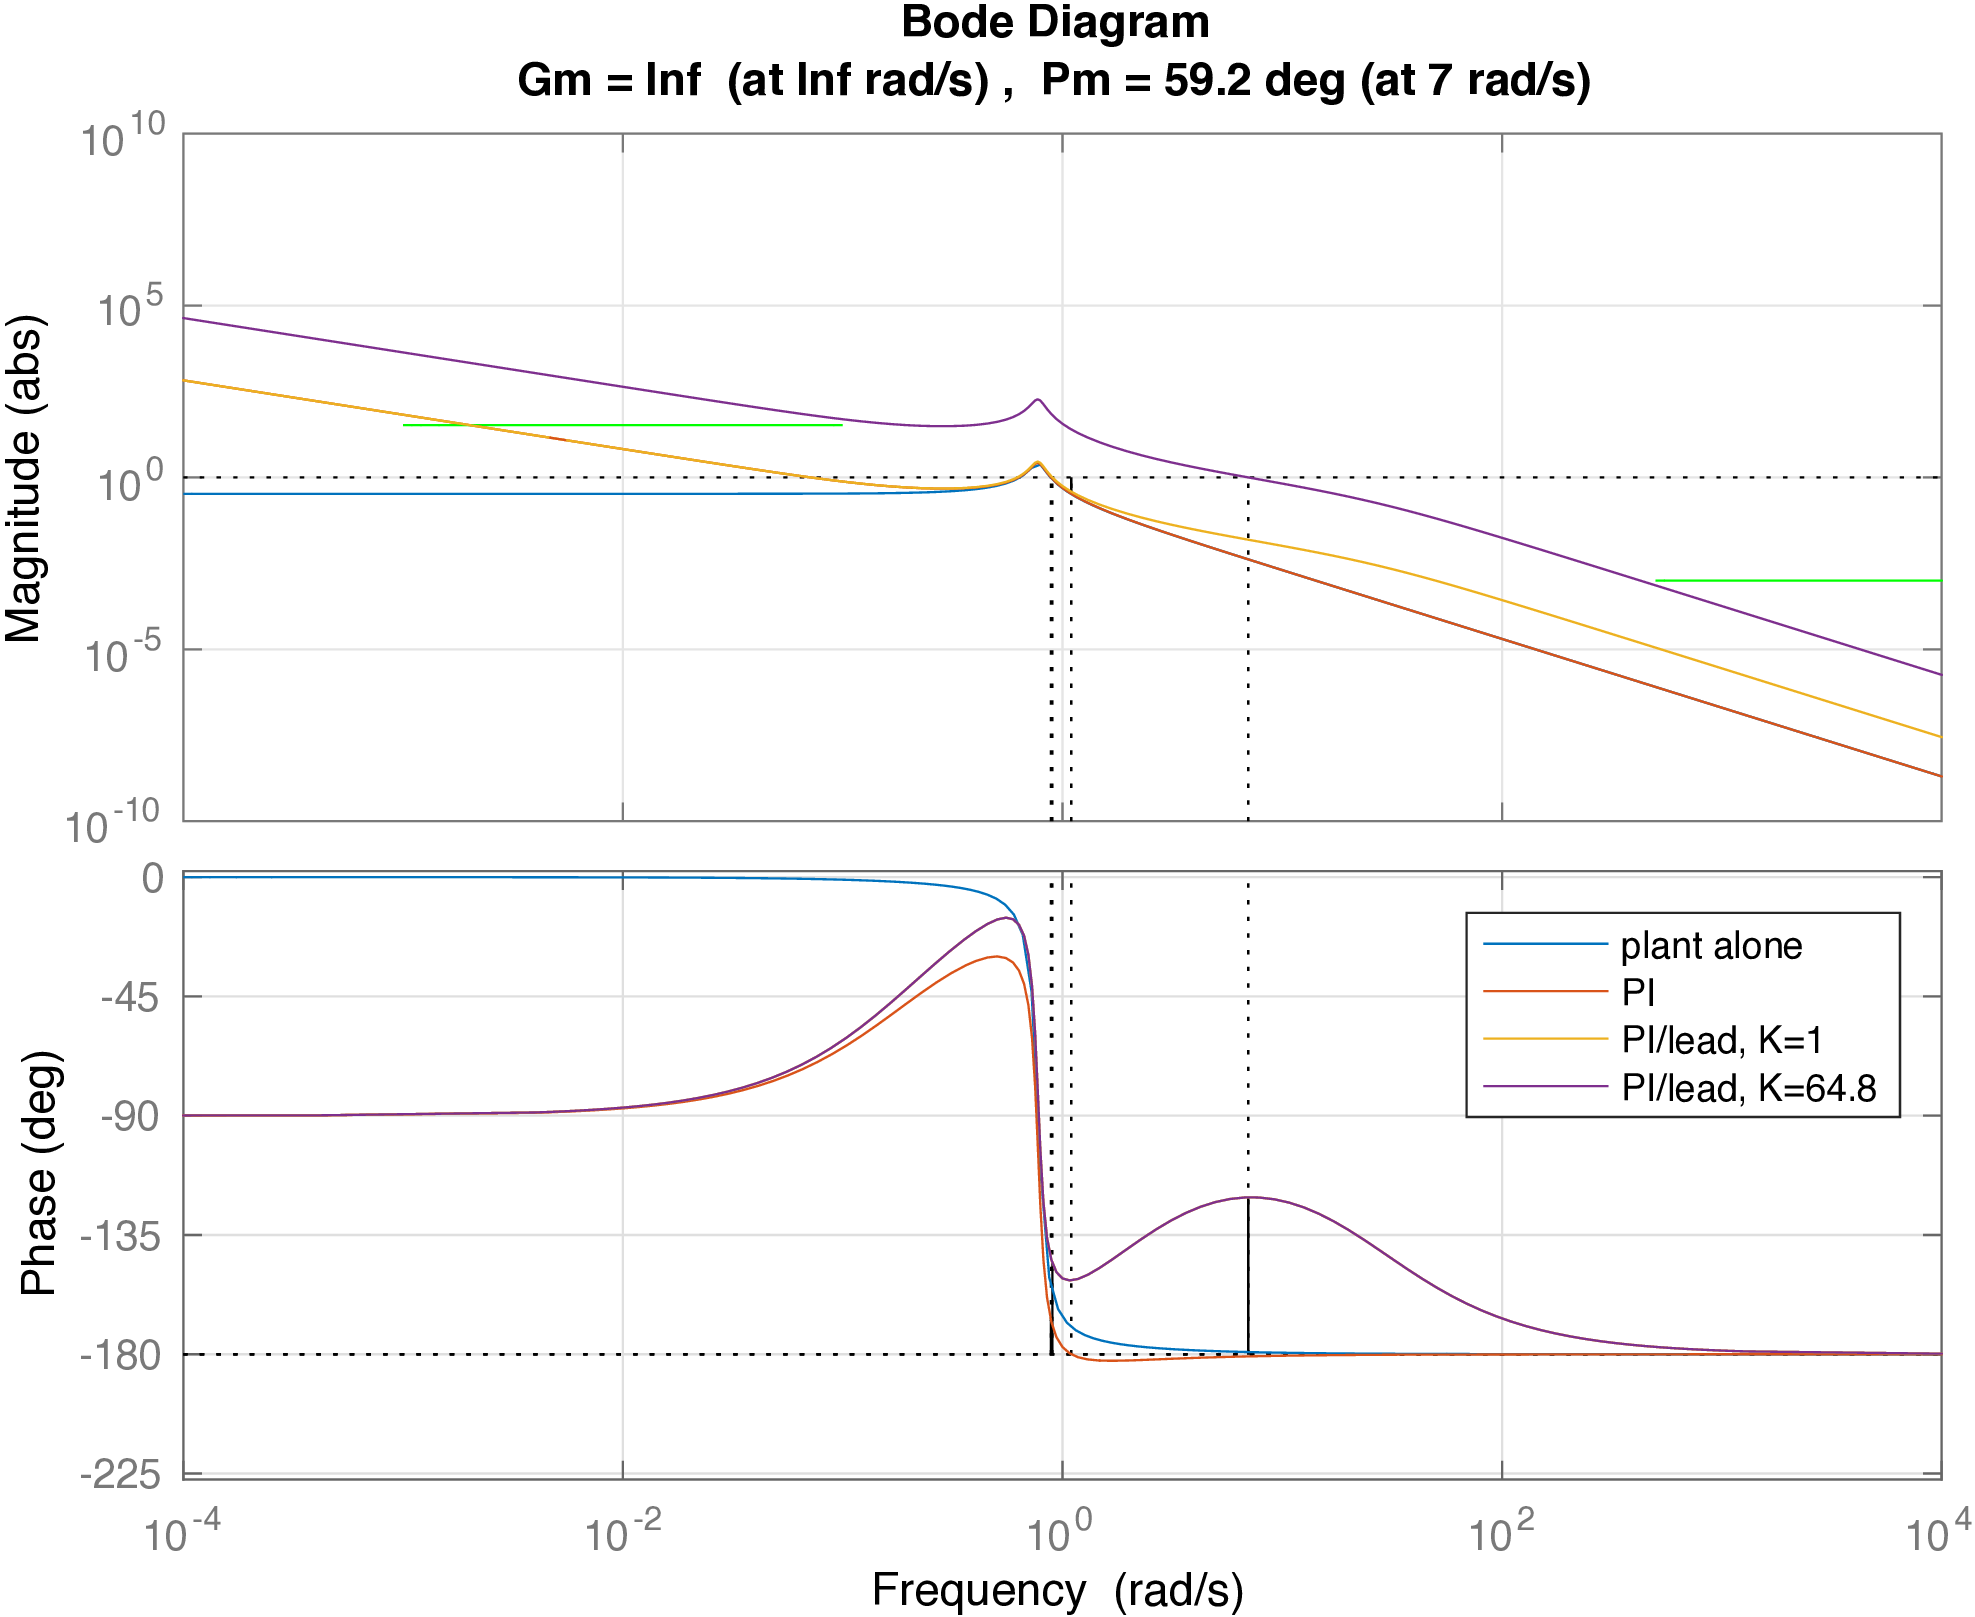
\includegraphics[width=0.95\textwidth]{6_design_studies/figures/hw_mass_compensator_design_3.pdf}
   \caption{The Bode plot for the system in HW~\ref{hw:mass}.\ref{chap:loopshaping_design}, with integral, phase lead, and proportional control.}
   \label{fig:hw_mass_compensator_design_3}
\end{figure}
%Noise attenuation is enhanced by adding the low pass filter
%\[
%C_{lpf} = \frac{50}{s+50}
%\]
%and the result is shown in Figure~\ref{fig:hw_mass_compensator_design_4}.
%\begin{figure}[H]
%   \centering
%   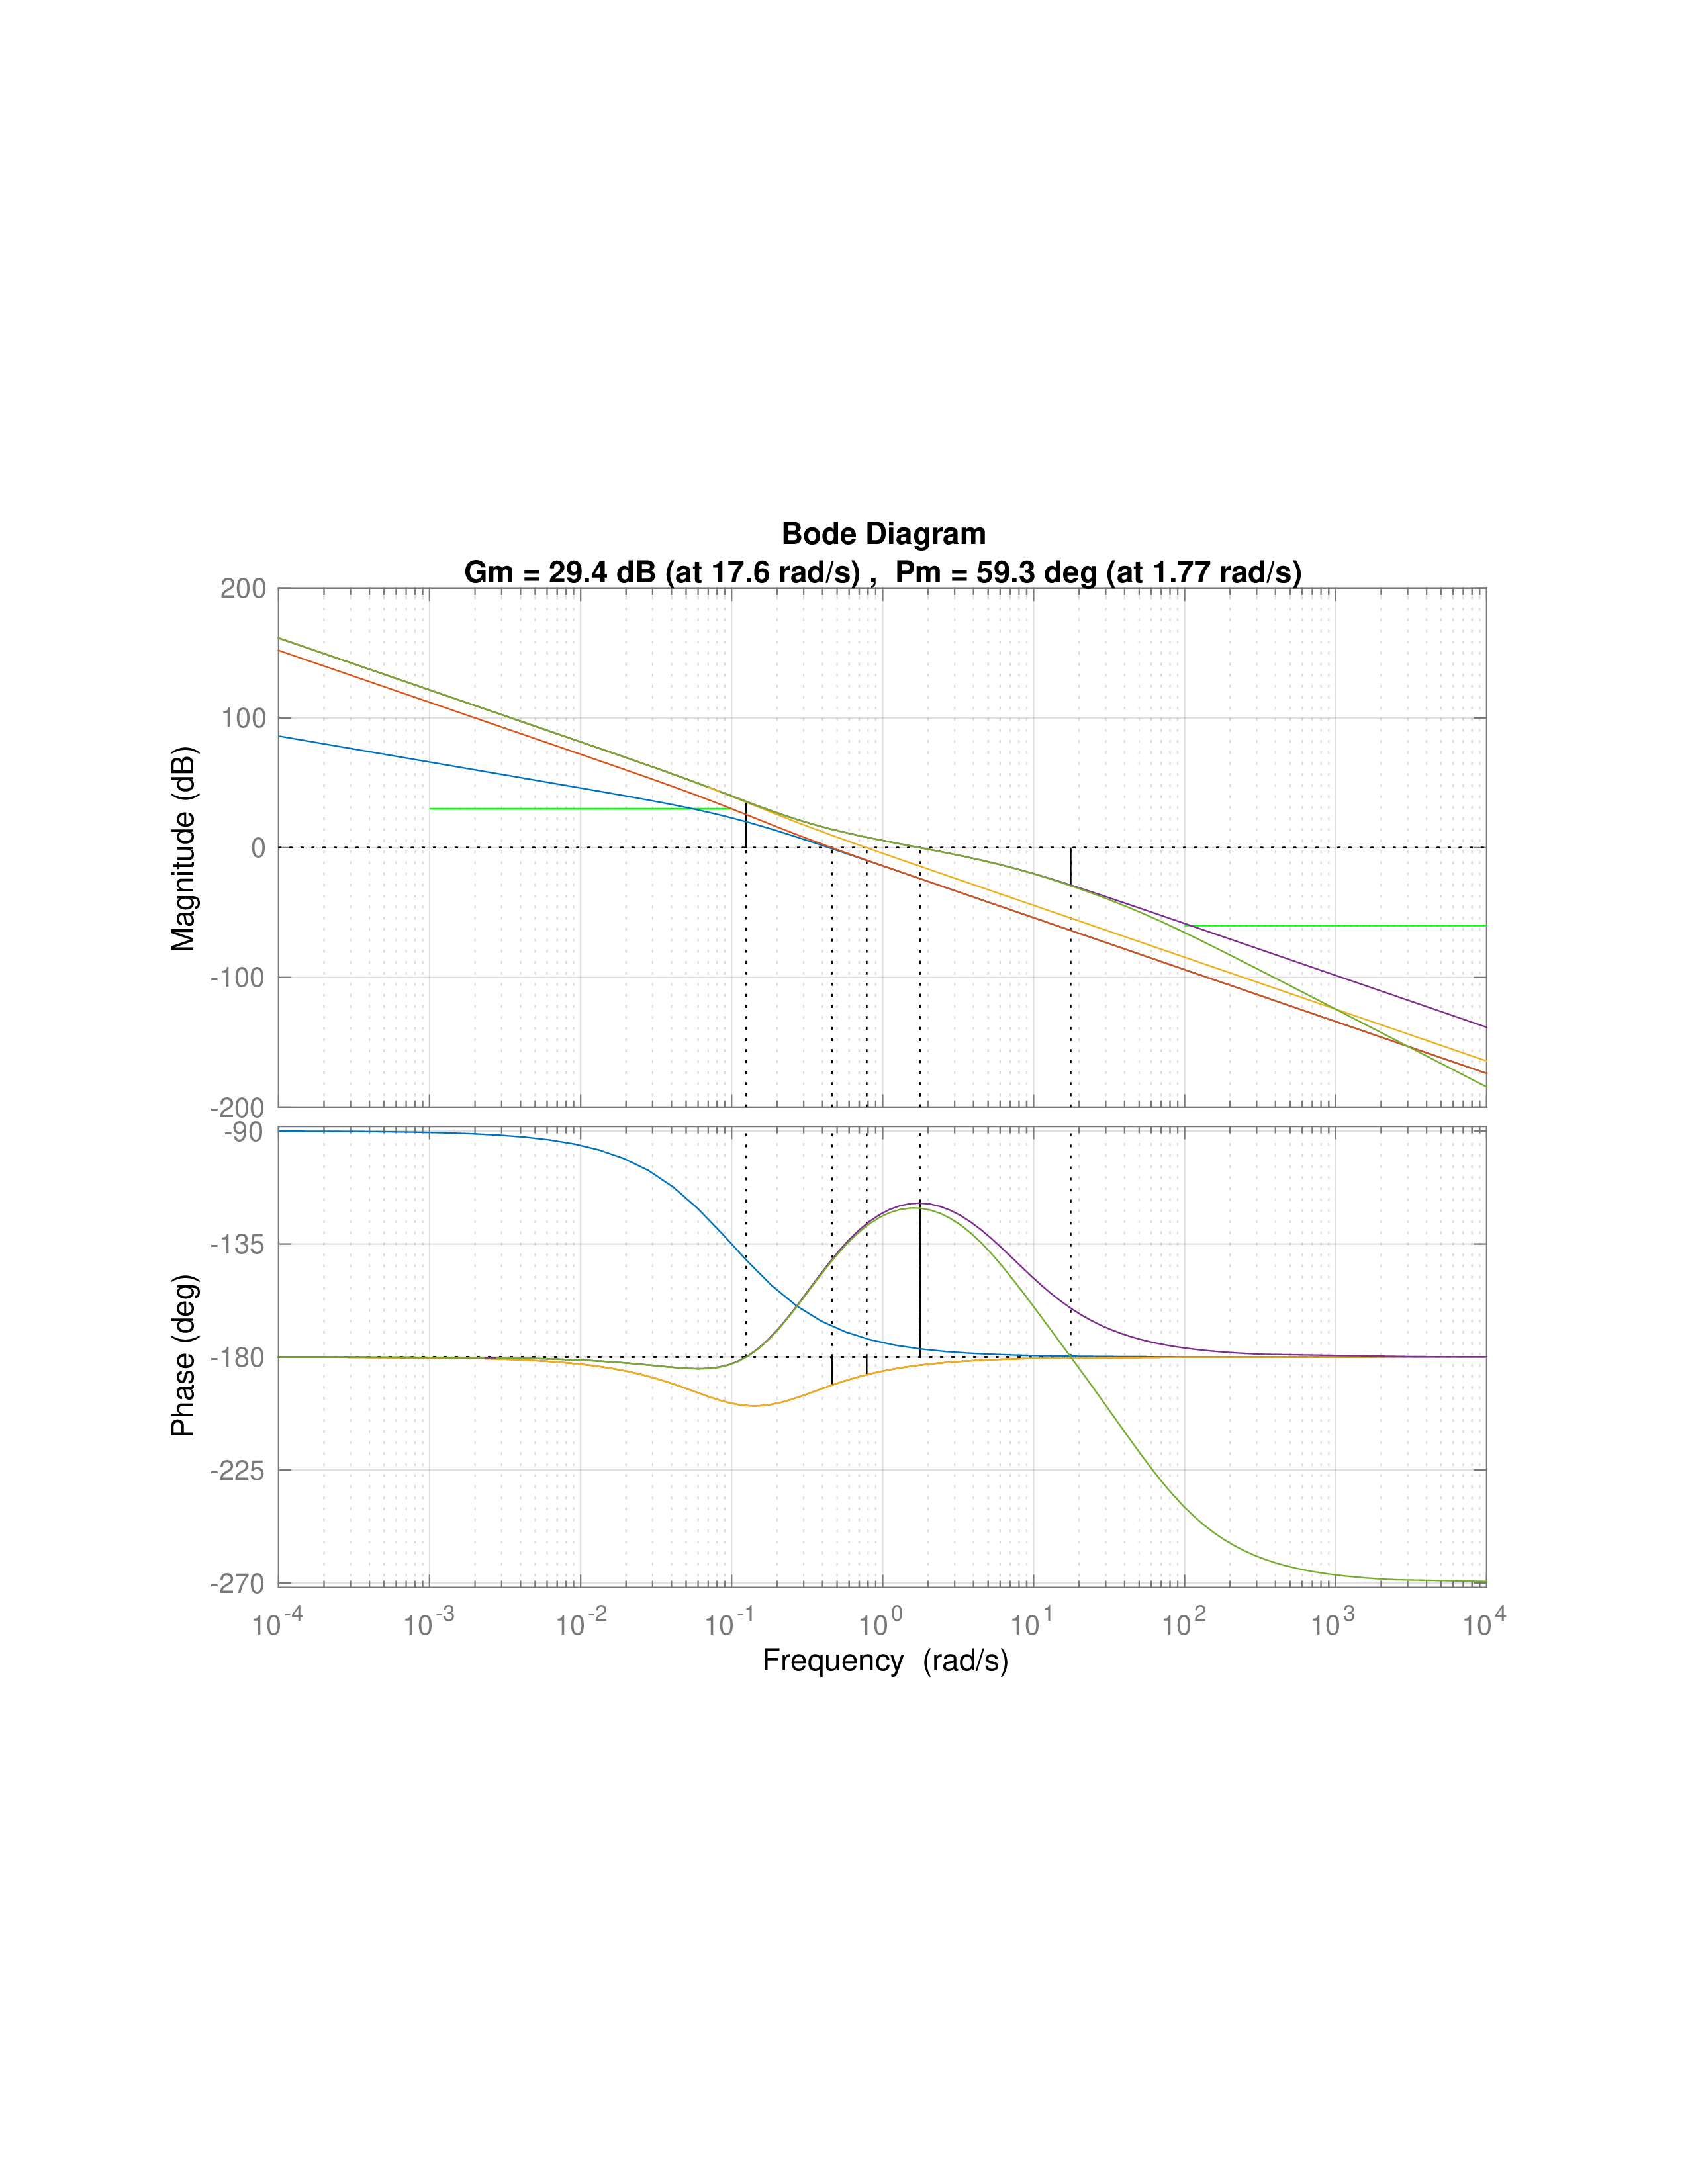
\includegraphics[width=0.95\textwidth]{6_design_studies/figures/hw_mass_compensator_design_4.pdf}
%   \caption{The Bode plot for the system in HW~\ref{ds:mass}.\ref{chap:loopshaping_design}, with with PI, phase lead, and proportional control.}
%   \label{fig:hw_mass_compensator_design_4}
%\end{figure}
%
Since the phase margin is $PM=59.2$~deg, we consider the phase margin specification to be satisfied.
The resulting compensator is
\[
C(s) = 903 \left(\frac{s+0.2}{s}\right)\left(\frac{s+1.88}{s+26.1}\right).
\]
The closed-loop response, 
as well as the unit-step response for the output and control signal are all show in Figure~\ref{fig:hw_mass_compensator_design_5}, where the prefilter
\[
F(s) = \frac{2}{s+2}
\]
has been added to reduce the peaking in the closed loop response.
\begin{figure}[H]
   \centering
   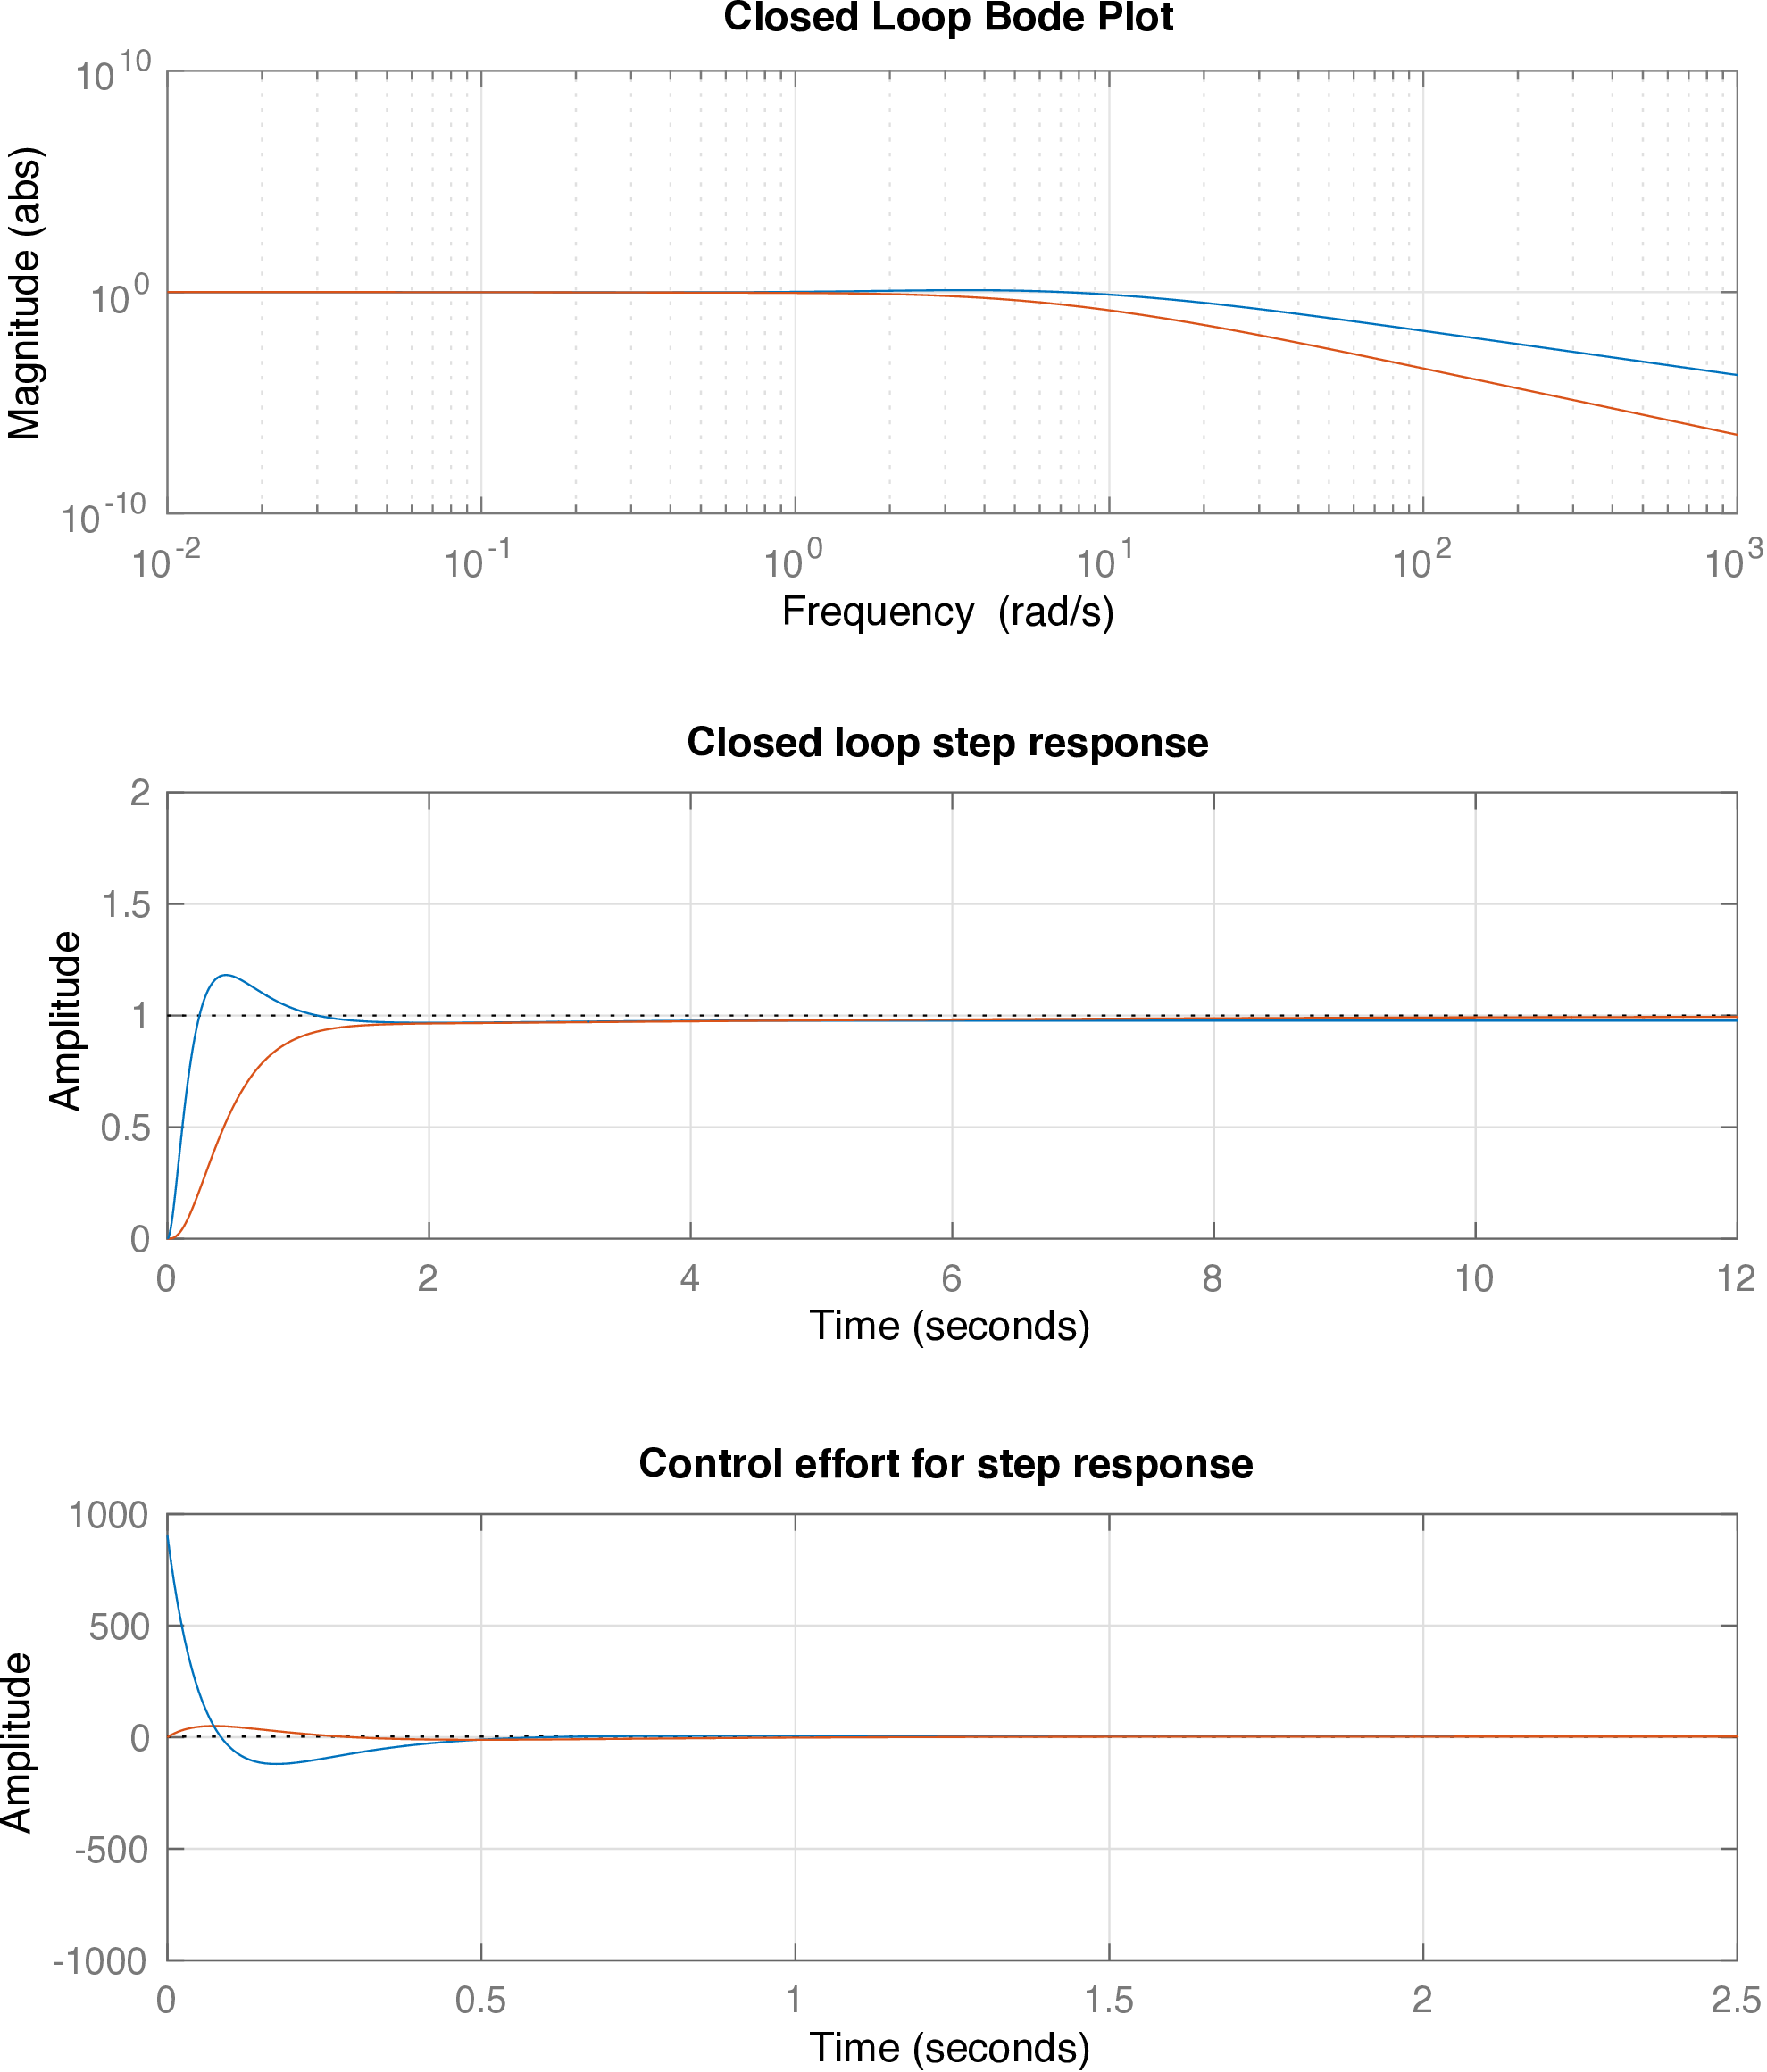
\includegraphics[width=0.95\textwidth]{6_design_studies/figures/hw_mass_compensator_design_5.pdf}
   \caption{The closed loop bode response, the unit step response for the output, and the unit step response for the input for the design in HW~\ref{hw:mass}.\ref{chap:loopshaping_design}.}
   \label{fig:hw_mass_compensator_design_5}
\end{figure}

The Matlab code used to design the outer loop is shown below.
\begin{lstlisting}

%%%%%%%%%%%%%%%%%%%%%%%%%%%%%%%%%%%%%%%%%%%%%%%%%%%%%%%%%%
  Define Design Specifications
%%%%%%%%%%%%%%%%%%%%%%%%%%%%%%%%%%%%%%%%%%%%%%%%%%%%%%%%%%

--- general tracking specification ---
    omega_r = 0.1;  % track signals below this frequency
    gamma_r = 0.03;  % tracking error below this value
    w = logspace(log10(omega_r)-2,log10(omega_r));

--- noise specification ---
    omega_n = 500;  % attenuate noise above this frequency
    gamma_n = 0.001;   % attenuate noise by this amount
    w = logspace(log10(omega_n),2+log10(omega_n));

%%%%%%%%%%%%%%%%%%%%%%%%%%%%%%%%%%%%%%%%%%%%%%%%%%%%%%%%%%
 Control Design
  C = tf(1,1);
%%%%%%%%%%%%%%%%%%%%%%%%%%%%%%%%%%%%%%%%%%%%%%%%%%%%%%%%%%

 integral control: 
     k_I = 0.2; % frequency at which integral action ends
     Integrator = tf([1,k_I],[1,0]);
     C = C*Integrator;

 phase lead: increase PM (stability)
     w_max = 7; % location of maximum frequency bump
     phi_max = 60*pi/180;
     M = (1+sin(phi_max))/(1-sin(phi_max)) % lead ratio
     z = w_max/sqrt(M)
     p = w_max*sqrt(M)
     Lead = tf([1/z 1],[1/p 1]);
     C = C*Lead;

 find gain to set crossover at w_max = 7 rad/s
     [m,p] = bode(C*Plant,w_max);
     K = 1/m;
     C = K*C;

%%%%%%%%%%%%%%%%%%%%%%%%%%%%%%%%%%%%%%%%%%%%%%%%%%%%%%%%%%
 Prefilter Design
     F = tf(1,1);
%%%%%%%%%%%%%%%%%%%%%%%%%%%%%%%%%%%%%%%%%%%%%%%%%%%%%%%%%%
   
 low pass filter
    p = 2;  % frequency to start the LPF
    LPF = tf(p, [1,p]);
    F = F*LPF;
        
%%%%%%%%%%%%%%%%%%%%%%%%%%%%%%%%%%%%%%%%%%%%%%%%%%%%%%%%%%
 Convert controller to state space equations 
%%%%%%%%%%%%%%%%%%%%%%%%%%%%%%%%%%%%%%%%%%%%%%%%%%%%%%%%%%
     [num,den] = tfdata(C,'v');
     [P.A_C,P.B_C,P.C_C,P.D_C]=tf2ss(num,den);

     [num,den] = tfdata(F,'v');
     [P.A_F, P.B_F, P.C_F, P.D_F] = tf2ss(num,den);
\end{lstlisting}

The complete Simulink files are on the wiki associated with the book.


